\subsection{Configuration editor}
\label{sec:arch-configuration}
\writer{Monica}

The Configuration Editor consists of only one class that links Petri net with its Geometry and Appearance.
In order to link them, the Configurator class contains references to all the above mentioned classes. 

Figure \ref{fig:uml-configuration-editor} shows the simple model behind the Configuration Editor and how all the information is gathered in order to run the simulation. 

\begin{figure}[htp]
\begin{center}
  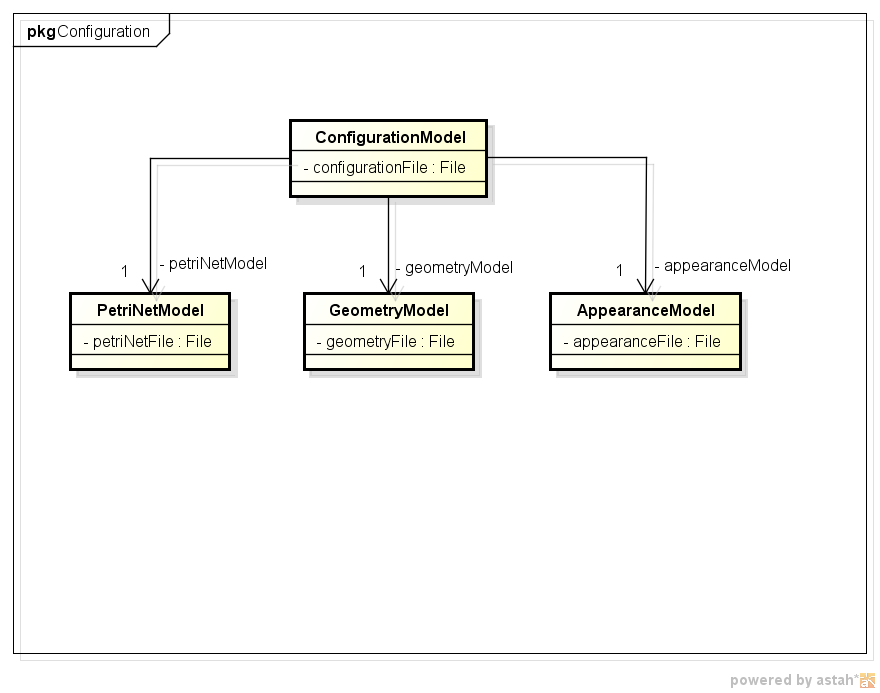
\includegraphics[width=0.8\textwidth]{image/configuration-model.png}
  \caption{UML for the Configuration Editor}
  \label{fig:uml-configuration-editor}
\end{center}
\end{figure}

After setting up all the references of the above mentioned files, the configuration will combine all of the and start the \textit{Simulator}. This can be done by pressing "Start simulation" in the pop-up menu when right-clicking the configuration object.
